\documentclass[11pt]{beamer}
\usepackage[utf8]{inputenc}
\usepackage[T1]{fontenc}
\usepackage{lmodern}
\usepackage[english]{babel}
\usepackage{graphicx}
\usepackage[most]{tcolorbox}
\usetheme{Darmstadt}
\setbeamertemplate{navigation symbols}{}
\setbeamertemplate{footline}{
	\begin{beamercolorbox}[ht=3ex,leftskip=1.4cm,rightskip=.3cm]{author in head/foot}
		\hfill \insertframenumber
		\vspace*{0.07cm}
	\end{beamercolorbox}
} 
\usepackage{url}
\usepackage{hyperref}
\usepackage{listings}

% color def
\usepackage{color}
\definecolor{darkred}{rgb}{0.6,0.0,0.0}
\definecolor{darkgreen}{rgb}{0,0.50,0}
\definecolor{lightblue}{rgb}{0.0,0.42,0.91}
\definecolor{orange}{rgb}{0.99,0.48,0.13}
\definecolor{grass}{rgb}{0.18,0.80,0.18}
\definecolor{pink}{rgb}{0.97,0.15,0.45}

\usepackage{nth}

% General Setting of listings
\lstset{
	language=Python,
	tabsize=4,
	aboveskip=1em,
	breaklines=true,
	abovecaptionskip=-6pt,
	captionpos=b,
	escapeinside={\%*}{*)},
	frame=single,
	numbers=left,
	numbersep=8pt,
	numberstyle=\tiny,
	morekeywords=[1]{,as,assert,nonlocal,with,yield,self,True,False,None,} % Python builtin
	morekeywords=[2]{,__init__,__add__,__mul__,__div__,__sub__,__call__,__getitem__,__setitem__,__eq__,__ne__,__nonzero__,__rmul__,__radd__,__repr__,__str__,__get__,__truediv__,__pow__,__name__,__future__,__all__,}, % magic methods
	morekeywords=[3]{,object,type,isinstance,copy,deepcopy,zip,enumerate,reversed,list,set,len,dict,tuple,range,xrange,append,execfile,real,imag,reduce,str,repr,}, % common functions
	morekeywords=[4]{,Exception,NameError,IndexError,SyntaxError,TypeError,ValueError,OverflowError,ZeroDivisionError,}, % errors
	morekeywords=[5]{,ode,fsolve,sqrt,exp,sin,cos,arctan,arctan2,arccos,pi, array,norm,solve,dot,arange,isscalar,max,sum,flatten,shape,reshape,find,any,all,abs,plot,linspace,legend,quad,polyval,polyfit,hstack,concatenate,vstack,column_stack,empty,zeros,ones,rand,vander,grid,pcolor,eig,eigs,eigvals,svd,qr,tan,det,logspace,roll,min,mean,cumsum,cumprod,diff,vectorize,lstsq,cla,eye,xlabel,ylabel,squeeze,}, % numpy / math
	deletekeywords=[2]{next,set},
	deletekeywords=[3]{next,set},
	basicstyle=\ttfamily\small,
	backgroundcolor=\color{white},
	commentstyle=\color{darkgreen}\slshape,
	keywordstyle=\color{blue}\bfseries\itshape,
	keywordstyle=[2]\color{blue}\bfseries,
	keywordstyle=[3]\color{grass},
	keywordstyle=[4]\color{red},
	keywordstyle=[5]\color{orange},
	stringstyle=\color{darkred},
	emphstyle=\color{pink}\underbar,
	morestring=*[d]{"},
}

\usepackage{tikz}
\usetikzlibrary{calc,shapes.multipart,chains,arrows,positioning}

\tikzset{
	squarecross/.style={
		draw, rectangle,minimum size=18pt, fill=orange!80,
		inner sep=0pt, text=black,
		path picture = {
			\draw[black]
			(path picture bounding box.north west) --
			(path picture bounding box.south east)
			(path picture bounding box.south west) --
			(path picture bounding box.north east);
		}
	},
	list/.style={
		very thick, rectangle split,
		rectangle split parts=2, draw,
		rectangle split horizontal, minimum size=18pt,
		inner sep=4pt, text=black,
		rectangle split part fill={red!20, blue!20}
	},
	->, start chain, very thick,
	chain_arrow/.style={*->, thick}
}


\begin{document}
	\author{Data Structures}
	\title{Computational Complexity \\
	\& \\
	Recursion}
	\titlegraphic{
\includegraphics[width=3cm]{img/UPNA}}
	\date[]{2023-2024}
	\subject{Data Structures}
	%\subtitle{}
	%\logo{}
	%\institute{}
	%\date{}
	%\subject{}
	%\setbeamercovered{transparent}
	%\setbeamertemplate{navigation symbols}{}
	\begin{frame}[plain]
		\maketitle
	\end{frame}

	\begin{frame}
		\tableofcontents
	\end{frame}

\section{Measuring Complexity}

\subsection{What is efficiency?}

\begin{frame}\frametitle{Algorithm efficiency}
\begin{itemize}
\item Several methods to implement a solution to a problem
\item How do we decide which one is the best?
\pause
\item The easiest to understand?
\pause
\item The one that needs less time?
\pause
\begin{itemize}
\item Will the algorithm that requires 1 second to analyse 10 data points require 10 seconds to analyse 100?
\end{itemize}
\end{itemize}
\end{frame}

\subsection{Experimental approach}

\begin{frame}[fragile]\frametitle{Using time to measure complexity}
\begin{lstlisting}
import time

def sum_smaller_than(n):
    the_sum = 0
    for i in range(n):
        the_sum += i
    return the_sum

start = time.time()
sum_smaller_than(10000000)
end = time.time()
print(f"The sum needed {end-start:.4} seconds")
# The sum needed 0.6202 seconds
\end{lstlisting}
\end{frame}

\begin{frame}[fragile]\frametitle{Repetitions are needed}
\begin{lstlisting}
# The sum needed 0.6202 seconds
# The sum needed 0.506 seconds
# The sum needed 0.468 seconds
# The sum needed 0.4748 seconds
# The sum needed 0.4771 seconds
# The sum needed 0.472 seconds
\end{lstlisting}
\begin{block}{}
\centering Why does the time decrease?
\end{block}
\pause
\begin{itemize}
\item Repeated measurements are needed and the results averaged
\item If we modify \texttt{n} how will the time needed change?
\end{itemize}
\end{frame}

\subsection{Formal approach}

\begin{frame}\frametitle{Mathematical analysis}
\begin{itemize}
\item Using the time needed to execute an algorithm may give us an idea of the efficiency of the algorithm
\pause
\item It is not comparable 
\begin{itemize}
\item Which programming language is used
\item Which computer is it running on
\end{itemize}
\pause
\item A formal approach is needed to define the complexity
\begin{itemize}
\item Time complexity
\item Space complexity
\end{itemize}
\end{itemize}
\end{frame}

\begin{frame}[fragile]\frametitle{Counting operations}
\begin{lstlisting}
def sum_smaller_than(n):
    the_sum = 0				# 1 operation
    for i in range(n):
        the_sum += i		# n operations
    return the_sum
\end{lstlisting}
\begin{itemize}
\item The most basic approach is to count how many operations are needed to execute the code
\end{itemize}
\pause
\begin{block}{}
\centering$T(n) = 1 + n$
\end{block}
\end{frame}


\begin{frame}\frametitle{Big O notation}
\begin{itemize}
\item Usually we are not interested in the specific expression, just an approximation
\item The Big O notation describes how an algorithms will grow
\item $8n^2 + 13n + 1324 \Rightarrow O(n^2)$
\end{itemize}
\begin{center}
\begin{tabular}{l|l}
\hline
\textbf{f(n)} & \textbf{Name} \\
\hline
1 &  Constant \\
log n & Logarithmic \\
n & Linear \\
n log n & Log Linear \\
$n^2$ & Quadratic \\
$n^3$ & Cubic \\
$2^n$ & Exponential \\
\end{tabular}
\end{center}
\end{frame}

\begin{frame}\frametitle{Big O chart}
\begin{figure}
\centering
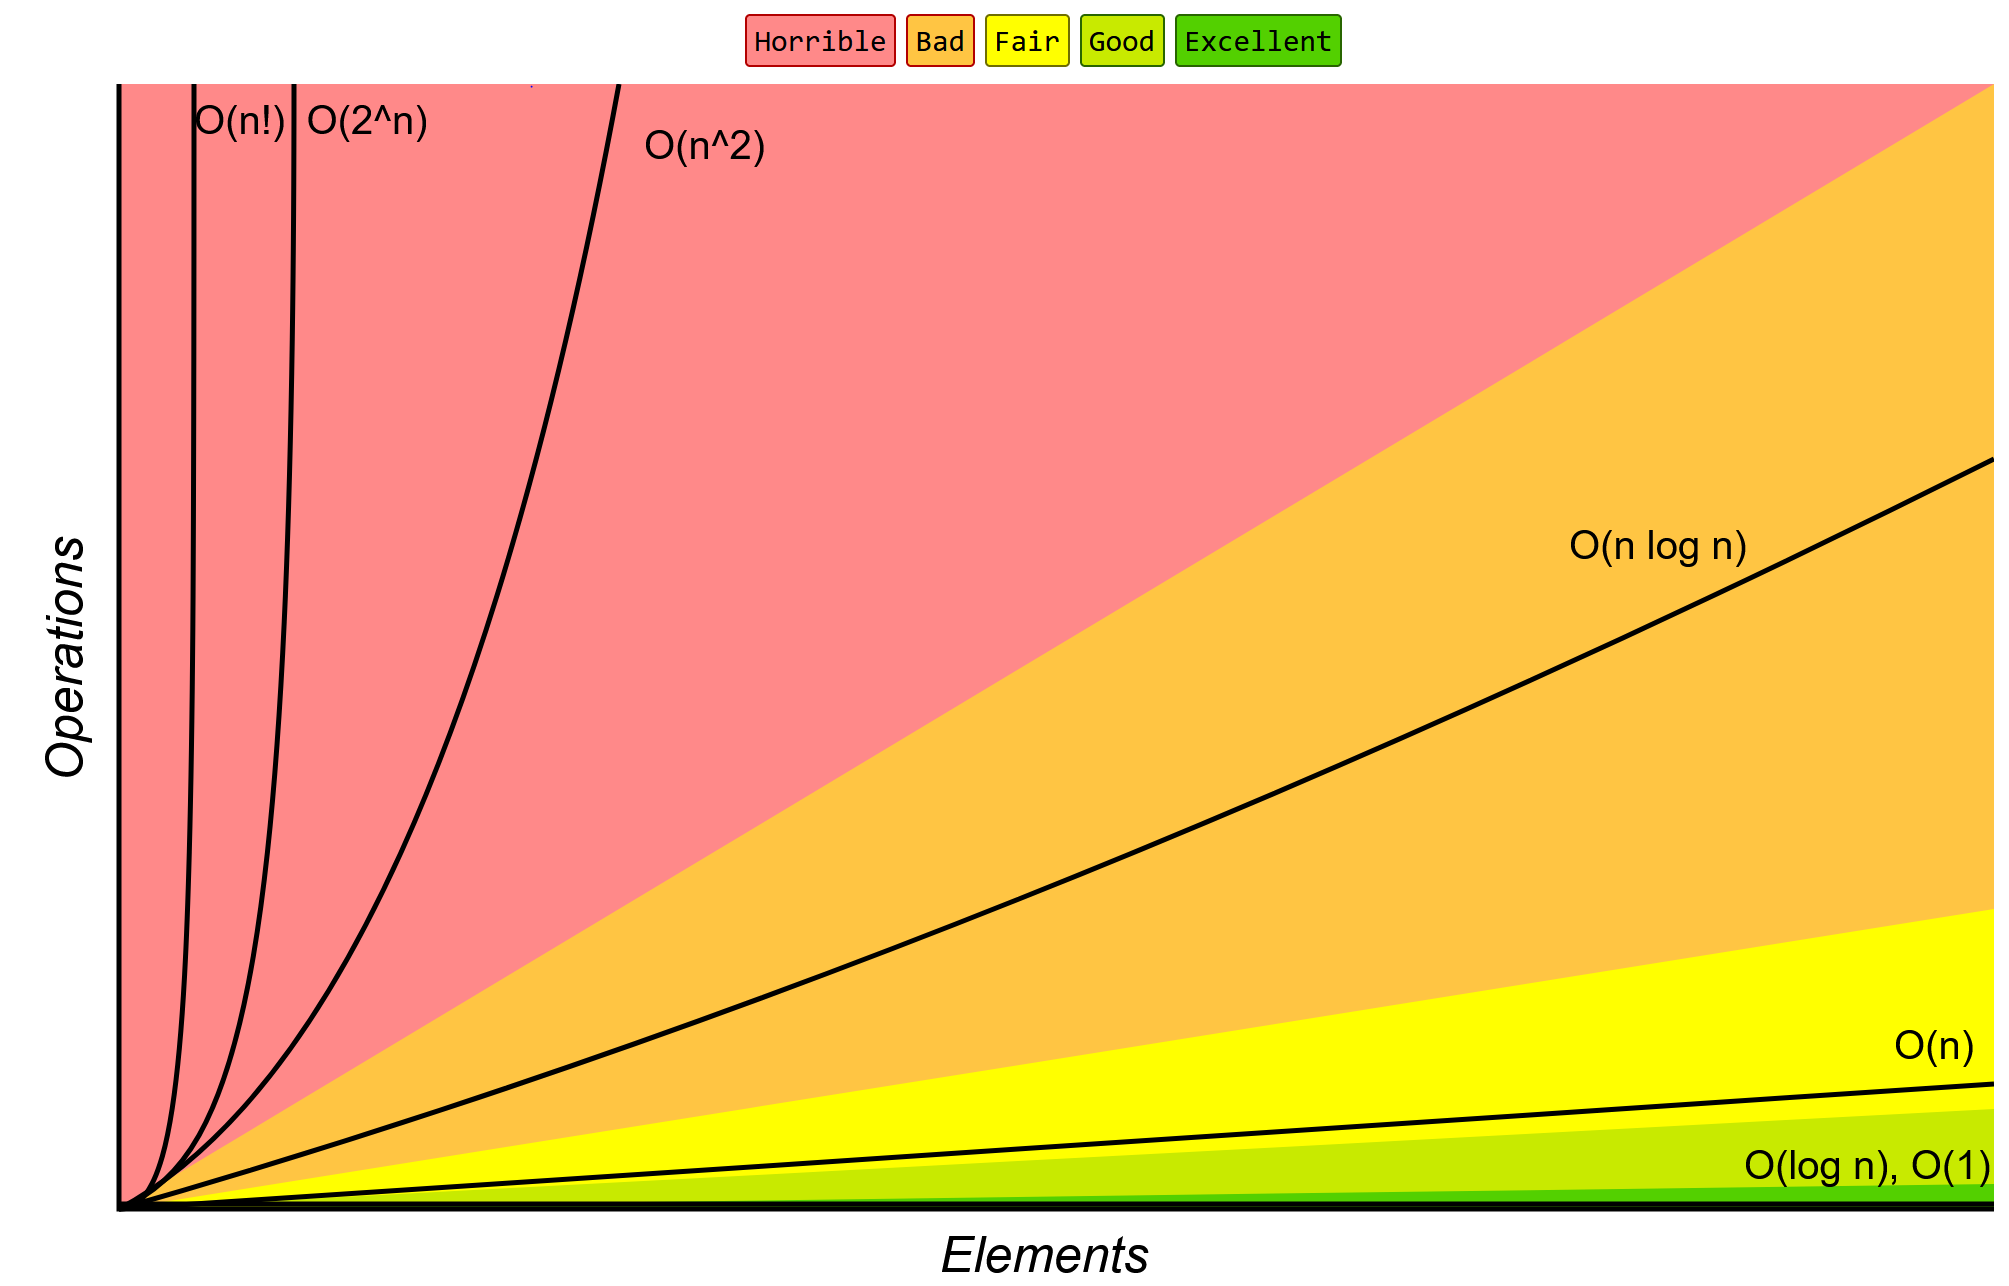
\includegraphics[width=0.9\linewidth]{img/bigo}
\label{fig:bigo}
\end{figure}
\href{https://www.bigocheatsheet.com/}{https://www.bigocheatsheet.com/}
\end{frame}

\subsection{Complexity exercises}

\begin{frame}[fragile, allowframebreaks]\frametitle{Example complexity}
\begin{lstlisting}
n = 1000
b = 2
c = 3
for i in range(n):
	for j in range(n):
		x = i * i
		y = j * j
		z = i * j
for k in range(n):
	w = c * k + 15
	v = b * b
d = 33
\end{lstlisting}
\framebreak
\begin{lstlisting}
n = 1000				# 1
b = 2					# 1
c = 3					# 1
for i in range(n):
	for j in range(n):
		x = i * i		# n^2
		y = j * j		# n^2
		z = i * j		# n^2
for k in range(n):
	w = c * k + 15		# n
	v = b * b			# n
d = 33					# 1
\end{lstlisting}
\begin{block}{}
\centering$T(n) = 3 + 3n^2 + 2n + 1 \rightarrow O(n^2)$
\end{block}
\end{frame}

\begin{frame}[fragile, allowframebreaks]\frametitle{List minimum}
\begin{block}{}
Write a function that returns the minimum value on a list of integers. What is its complexity?
\end{block}
\framebreak
\begin{lstlisting}
def lst_min(lst):
	return min(lst) # what is the complexity of min()?
\end{lstlisting}
\begin{block}{}
\centering $O(?)$
\end{block}
\framebreak
\begin{lstlisting}
def lst_min(lst):
	minimum = lst[0]			# 1
	for value in lst:
		if value < minimum:		# n
			minimum = value		# less than n
	return minimum
\end{lstlisting}
\begin{block}{}
\centering $O(n)$
\end{block}
\end{frame}

\colorlet{lightgreen}{green!60!}

\tcbset{on line, 
        boxsep=4pt, left=0pt,right=0pt,top=0pt,bottom=0pt,
        colframe=white,colback=lightgreen,  
        highlight math style={enhanced}
        }

\begin{frame}[fragile]\frametitle{Exercise 1}
\begin{lstlisting}
test = 0
for i in range(n):
	for j in range(n):
		test = test + i * j
\end{lstlisting}
\begin{enumerate}
\item $O(n)$
\item \alt<2>{\tcbox{$O(n^2)$}}{$O(n^2)$}
\item $O(log\ n)$
\item $O(n^3)$
\end{enumerate}
\end{frame}

\begin{frame}[fragile]\frametitle{Exercise 2}
\begin{lstlisting}
test = 0
for i in range(n):
	test = test + 1
	
for j in range(n):
	test = test + 1
\end{lstlisting}
\begin{enumerate}
\item \alt<2>{\tcbox{$O(n)$}}{$O(n)$}
\item $O(n^2)$
\item $O(log\ n)$
\item $O(n^3)$
\end{enumerate}
\end{frame}

\begin{frame}[fragile]\frametitle{Exercise 3}
\begin{lstlisting}
i = n
while i > 0:
	k = 2 + 2
	i = i // 2
\end{lstlisting}
\begin{enumerate}
\item $O(n)$
\item $O(n^2)$
\item  \alt<2>{\tcbox{$O(log\ n)$}}{$O(log\ n)$}
\item $O(n^3)$
\end{enumerate}
\end{frame}

\subsection{Complexity of common structures}

\begin{frame}\frametitle{Efficiency of Python lists}
\begin{center}
\begin{tabular}{l|l}
\hline
\textbf{Operation} &\textbf{ Big O Efficiency} \\
\hline
get & $O(1)$ \\
set & $O(1)$ \\
append & $O(1)$ \\
insert(i, item) & $O(n)$ \\
pop() & $O(1)$ \\
pop(i) & $O(n)$ \\
del & $O(n)$ \\
contains & $O(n)$ \\
reverse & $O(n)$ \\
sort & $O(n\ log\ n)$ \\
multiply & $O(nk)$ \\
\end{tabular}
\end{center}
\end{frame}


\begin{frame}\frametitle{Efficiency of Python dictionaries}
\begin{center}
\begin{tabular}{l|l}
\hline
\textbf{Operation} &\textbf{ Big O Efficiency} \\
\hline
get & $O(1)$ \\
set & $O(1)$ \\
del & $O(1)$ \\
contains & $O(1)$ \\
copy & $O(n)$ \\
\end{tabular}
\end{center}
\end{frame}

\section{Recursion}

\begin{frame}{Overview}
\tableofcontents[currentsection,hideothersubsections]
\end{frame}

\subsection{What is recursion?}
\begin{frame}\frametitle{Recursion}
\begin{block}{}
Recursion is the process of repeating items in a self-similar way
\end{block}
\begin{description}
\item[Algorithmically:] a way to design solutions to problems by divide-and-conquer or decrease-and-conquer
\begin{itemize}
\item Reduce a problem to simpler versions of the same problem
\end{itemize}
\item[Semantically:] a programming technique where a function calls itself
\begin{itemize}
\item Solve the same problem on some other input with the goal of simplifying the larger problem input
\end{itemize}
\end{description}
\end{frame}

\begin{frame}\frametitle{Iterative VS recursive algorithms}
\begin{itemize}
\item Looping statements (\texttt{while} and \texttt{for} loops) lead to iterative algorithms
\begin{itemize}
\item Compute using a set of state variables that update on each iteration of the loops
\end{itemize}
\item Recursion is able to create loops without the need of iterative approaches
\end{itemize}
\end{frame}

\subsection{Recursion by example}

\begin{frame}[fragile]\frametitle{Multiplication - Iterative}
\begin{block}{}
\centering $a \times b$ is equivalent to add a to itself b times
\end{block}
\begin{lstlisting}
def multiply_iter(a, b):
	result = 0
	for i in range(b):
		result += a
	return result
\end{lstlisting}
\end{frame}

\begin{frame}[fragile]\frametitle{Multiplication - Recursive}
\begin{block}{Reduce the problem to a smaller one}
\centering $a \times b$ is equivalent to $a + (a  \times (b - 1))$
\end{block}
\begin{block}{Base case}
\centering when $b = 1$ then $a \times b = a$
\end{block}
\pause
\begin{lstlisting}
def multiply_recur(a, b):
	if b == 1:
		return a
	else:
		return a + multiply_recur(a, b - 1)
\end{lstlisting}
\end{frame}

\begin{frame}[fragile]\frametitle{Factorial}
\begin{block}{}
\centering $n! = n \times (n - 1) \times (n - 2) \times (n - 3) \times \ldots \times 1$
\end{block}
\begin{description}
\item[Base case:] We know that the factorial of 1 is 1
\item[Reduce the problem:] The factorial of n is $n \times (n - 1)!$
\end{description}
\pause
\begin{lstlisting}
def fact(n):
	if n == 1:
		return n
	else:
		return n * fact(n-1)
\end{lstlisting}
\end{frame}

\subsection{Rules}

\begin{frame}\frametitle{Recursion characteristics}
\begin{itemize}
\item In some cases the recursion might be simpler and more intuitive
\item Recursion may be efficient from a programmer's point of view
\item Recursion may not be efficient from a computer's point of view
\begin{block}{}
Recursion needs to create a call stack for the recursive calls, and keep those variables in memory. It is easy to create an algorithm that is not efficient.
\end{block}
\end{itemize}
\end{frame}

\begin{frame}\frametitle{Summary}
\begin{itemize}
\item All recursive algorithms have a base case
\item All recursive algorithms must change their state (on each recursion) and get closer to the base case
\item A recursive algorithm is an algorithm that calls itself
\end{itemize}
\end{frame}

\subsection{Exercises}

\begin{frame}\frametitle{Sum elements on a list}
\begin{block}{Create a recursive algorithm that returns the sum of all elements on a list}
Do not use the \texttt{sum()} function
\end{block}
\begin{block}{How many calls are needed to calculate the sum of the following lists?}
\texttt{[3, 4, 6, 8, 0, 10, 11]} \\
\texttt{['3']} \\
\texttt{[]}
\end{block}
\end{frame}


\begin{frame}[fragile]\frametitle{Sum elements on a list: solution}
\begin{lstlisting}
def list_sum(lst):
    if len(lst) == 1:
        return lst.pop()
    else:
        return lst.pop() + list_sum(lst)
\end{lstlisting}
\end{frame}

\begin{frame}\frametitle{The Fibonacci sequence}
\begin{itemize}
\item The Fibonacci sequence is defined by the following equations:
\begin{equation*}
\begin{aligned}
f_0 &= 0\\
f_1 &= 1\\
f_n &= f_{n-1} + f_{n-2}
\end{aligned}
\end{equation*}
\item Implement a recursive algorithm to obtain any number in the Fibonacci sequence
\end{itemize}
\end{frame}

\begin{frame}[fragile]\frametitle{The Fibonacci sequence: solution}
\begin{lstlisting}
def fibonacci(n):
	if n == 0:
		return 0
	elif n == 1:
		return 1
	else:
		return fibonacci(n-1) + fibonacci(n-2)
\end{lstlisting}
\begin{block}{Efficiency}
The solution shown here is highly inefficient, try to calculate the \nth{10}, \nth{20} and \nth{30} Fibonacci numbers, did the time increase linearly?\\
How can we improve it?
\end{block}
\end{frame}

\begin{frame}\frametitle{Reverse a list in place}
\begin{block}{Create a function that is able to reverse a list in a recursive manner}
The list should be reversed in place. This means that no lists can be created and list slicing is not allowed.
\end{block}
\begin{description}
\item[A small tip:] The function you create will not take just the list, but also the start and end indexes to exchange. On each iteration swap the values of the start and end indexes and modify them accordingly
\end{description}
\end{frame}


%\begin{frame}[fragile]\frametitle{Reverse a list in place: solution}
%\begin{lstlisting}
%def reverse(lst, start, end):
%    if start > end: 
%        return lst
%    else:
%        lst[start], lst[end] = lst[end], lst[start]
%        start += 1
%        end -= 1
%        return reverse(lst, start, end)
%\end{lstlisting}
%\end{frame}

\end{document}






